    \begin{tikzpicture}[scale=1.5, >=latex]
        % Define cube dimensions
        \def\dx{2}
        \def\dy{2}
        \def\dz{1.5}

        % Coordinates
        \coordinate (O) at (0,0,0);
        \coordinate (A) at (\dx,0,0);
        \coordinate (B) at (\dx,\dy,0);
        \coordinate (C) at (0,\dy,0);
        \coordinate (D) at (0,0,\dz);
        \coordinate (E) at (\dx,0,\dz);
        \coordinate (F) at (\dx,\dy,\dz);
        \coordinate (G) at (0,\dy,\dz);

        % --- HIDDEN EDGES (Back) ---
        \draw[dashed] (O) -- (A);
        \draw[dashed] (O) -- (C);
        \draw[dashed] (O) -- (D);

        % --- INFLOW ARROWS ---
        \draw[->, thick, blue] (-1, \dy/2, \dz/2) -- (0, \dy/2, \dz/2) node[midway, above] {$\rho u$};
        \draw[->, thick, blue] (\dx/2, -1, \dz/2) -- (\dx/2, 0, \dz/2) node[midway, right] {$\rho v$};
        \draw[->, thick, blue] (\dx/2, \dy/2, -1) -- (\dx/2, \dy/2, 0) node[midway, right] {$\rho w$};

        % --- VISIBLE EDGES ---
        \draw[thick] (A) -- (B) -- (F) -- (E) -- cycle; % Right Face
        \draw[thick] (C) -- (B) -- (F) -- (G) -- cycle; % Top Face
        \draw[thick] (D) -- (E) -- (F) -- (G) -- cycle; % Front Face
        \draw[thick] (C) -- (G) -- (D);

        % --- OUTFLOW ARROWS ---
        \draw[->, thick, red] (\dx, \dy/2, \dz/2) -- (\dx+1.5, \dy/2, \dz/2) node[right] {$\rho u + \dfrac{\partial (\rho u)}{\partial x}dx$};
        \draw[->, thick, red] (\dx/2, \dy, \dz/2) -- (\dx/2, \dy+1.2, \dz/2) node[above] {$\rho v + \dfrac{\partial (\rho v)}{\partial y}dy$};
        \draw[->, thick, red] (\dx/2, \dy/2, \dz) -- (\dx/2, \dy/2, \dz+3.2) node[below left] {$\rho w + \dfrac{\partial (\rho w)}{\partial z}dz$};

        % --- AXES ---
        \draw[->, thick] (\dx+1, -1, \dz) -- (\dx+2, -1, \dz) node[right] {$x$};
        \draw[->, thick] (\dx+1, -1, \dz) -- (\dx+1, 0, \dz) node[above] {$y$};
        \draw[->, thick] (\dx+1, -1, \dz) -- (\dx+1, -1, \dz+1.5) node[left] {$z$};

        % --- DIMENSION LABELS ---
        \node at (\dx/2, -.2, \dz+0.1) {$dx$};
        \node at (-.1, \dy/2, \dz+0.3) {$dy$};
        \node at (\dx+0.3, 0, \dz/2) {$dz$};
    \end{tikzpicture}
